\documentclass[12pt,a4paper]{article}

% ─── Page Layout ───────────────────────────────────────────────────────────────
\usepackage[a4paper, margin=0.8in, headheight=14pt]{geometry}

% ─── Fonts (XeLaTeX) ───────────────────────────────────────────────────────────
\usepackage{fontspec}
\usepackage{unicode-math}
\setmainfont{TeX Gyre Pagella}
\setmonofont[Scale=0.88]{TeX Gyre Cursor}
\setmathfont{Latin Modern Math}

% ─── Packages ──────────────────────────────────────────────────────────────────
\usepackage{xcolor}
\usepackage{colortbl}
\usepackage{titlesec}
\usepackage{enumitem}
\usepackage{tabularx}
\usepackage{booktabs}
\usepackage{array}
\usepackage{amsmath}
\usepackage{tikz}
\usetikzlibrary{shapes.geometric, arrows.meta, positioning, calc, fit}
\usepackage{tcolorbox}
\tcbuselibrary{skins, breakable}
\usepackage{hyperref}
\usepackage{fancyhdr}
\usepackage{graphicx}
\usepackage{microtype}
\hyphenpenalty=10000
\exhyphenpenalty=10000
\sloppy
\usepackage{caption}
\usepackage{setspace}
\usepackage{multirow}
\usepackage{tocloft}

% ─── Q&A helper ────────────────────────────────────────────────────────────────
\newcommand{\Q}[1]{\textbf{#1}\par\noindent\ignorespaces}

% ─── Colour Palette ────────────────────────────────────────────────────────────
\definecolor{myred}{RGB}{196,30,58}
\definecolor{mydark}{RGB}{30,30,50}
\definecolor{mygreen}{RGB}{14,120,80}
\definecolor{myteal}{RGB}{0,130,140}
\definecolor{myamber}{RGB}{180,100,0}
\definecolor{mypurple}{RGB}{100,30,160}
\definecolor{mygray}{RGB}{246,247,249}
\definecolor{mgframe}{RGB}{180,185,200}
\definecolor{watermark}{RGB}{145,150,170}
\definecolor{hdrred}{RGB}{250,232,235}
\definecolor{hdrgreen}{RGB}{220,244,233}
\definecolor{hdrteal}{RGB}{220,242,244}
\definecolor{hdramber}{RGB}{253,242,215}
\definecolor{hdrpurple}{RGB}{238,228,255}
\definecolor{hdrgray}{RGB}{238,240,245}
\definecolor{rowalt}{RGB}{250,251,253}

% ─── Section Formatting ────────────────────────────────────────────────────────
\titleformat{\section}
  {\large\bfseries\color{myred}}{\thesection.}{0.5em}{}
  [\vspace{1pt}{\color{myred}\rule{\linewidth}{0.8pt}}]
\titleformat{\subsection}
  {\normalsize\bfseries\color{myteal}}{\thesubsection}{0.5em}{}
\titlespacing*{\section}{0pt}{18pt}{7pt}
\titlespacing*{\subsection}{0pt}{11pt}{4pt}

\setlength{\parindent}{0pt}
\setlength{\parskip}{4pt}

% ─── TOC Styling ───────────────────────────────────────────────────────────────
\renewcommand{\cfttoctitlefont}{\large\bfseries\color{myred}}
\renewcommand{\cftaftertoctitle}{\par\noindent{\color{myred}\rule{\linewidth}{0.8pt}}}
\setlength{\cftbeforetoctitleskip}{0pt}
\setlength{\cftaftertoctitleskip}{6pt}
\renewcommand{\cftsecfont}{\normalsize\bfseries\color{mydark}}
\renewcommand{\cftsecpagefont}{\normalsize\bfseries\color{mydark}}
\renewcommand{\cftsecleader}{\cftdotfill{\cftdotsep}}
\setlength{\cftbeforesecskip}{7pt}
\renewcommand{\cftsubsecfont}{\small\color{mydark}}
\renewcommand{\cftsubsecpagefont}{\small\color{mydark}}
\setlength{\cftbeforesubsecskip}{3pt}
\setlength{\cftsubsecindent}{1.4em}

% ─── Table helpers ─────────────────────────────────────────────────────────────
\renewcommand{\arraystretch}{1.45}
\setlength{\tabcolsep}{6pt}
\arrayrulecolor{mydark}
\newcolumntype{B}[1]{>{\small\bfseries\raggedright\arraybackslash}m{#1}}
\renewcommand{\tabularxcolumn}[1]{m{#1}}

% ─── Header / Footer ───────────────────────────────────────────────────────────
\pagestyle{fancy}
\fancyhf{}
\fancyhead[L]{\small\color{myred}\textbf{EC601}\;\color{mydark}--- Control System}
\fancyhead[R]{\small\color{myteal}\textbf{Module 5 Notes}}
\fancyfoot[C]{\small\color{mydark}\thepage}
\fancyfoot[R]{\small\color{watermark}\textit{\copyright\ Biraj}}
\renewcommand{\headrulewidth}{0.5pt}
\renewcommand{\footrulewidth}{0.3pt}

% ─── Hyperref ──────────────────────────────────────────────────────────────────
\hypersetup{
  colorlinks=true, linkcolor=myteal, urlcolor=myteal,
  pdfauthor={Biraj Sarkar},
  pdftitle={EC601 --- Module 5 Notes}
}

% ─── tcolorbox styles ──────────────────────────────────────────────────────────
\tcbset{
  tikzbox/.style={
    colback=mygray, colframe=mgframe, boxrule=0.6pt, arc=4pt,
    left=8pt, right=8pt, top=6pt, bottom=6pt,
    colbacktitle=mgframe, coltitle=mydark, fonttitle=\small\bfseries
  },
  defbox/.style={
    colback=hdrgreen, colframe=mygreen, boxrule=0.8pt, arc=4pt,
    left=9pt, right=9pt, top=6pt, bottom=6pt,
    colbacktitle=mygreen, coltitle=white, fonttitle=\small\bfseries
  },
  formulabox/.style={
    colback=hdrteal, colframe=myteal, boxrule=0.8pt, arc=4pt,
    left=9pt, right=9pt, top=7pt, bottom=7pt,
    colbacktitle=myteal, coltitle=white, fonttitle=\small\bfseries
  },
  examplebox/.style={
    colback=hdramber, colframe=myamber, boxrule=0.8pt, arc=4pt,
    left=9pt, right=9pt, top=6pt, bottom=6pt,
    colbacktitle=myamber, coltitle=white, fonttitle=\small\bfseries
  },
  masonbox/.style={
    colback=hdrpurple, colframe=mypurple, boxrule=0.8pt, arc=4pt,
    left=9pt, right=9pt, top=6pt, bottom=6pt,
    colbacktitle=mypurple, coltitle=white, fonttitle=\small\bfseries
  },
  exambox/.style={
    colback=hdrpurple, colframe=mypurple, boxrule=1pt, arc=5pt,
    left=10pt, right=10pt, top=8pt, bottom=8pt,
    colbacktitle=mypurple, coltitle=white, fonttitle=\bfseries,
    breakable, title after break={\textbf{Frequently Asked / Viva Questions (contd.)}}}
}
% Allow all boxes to break across pages
\tcbset{breakable}

% ─── TikZ styles ───────────────────────────────────────────────────────────────
\tikzset{
  block/.style={rectangle, draw=myteal, fill=hdrteal,
    text width=2.6cm, align=center, minimum height=0.95cm,
    font=\small, rounded corners=3pt, line width=0.7pt},
  redblock/.style={rectangle, draw=myred, fill=hdrred,
    text width=2.4cm, align=center, minimum height=0.95cm,
    font=\small, rounded corners=3pt, line width=0.7pt},
  sumjunc/.style={circle, draw=myamber, fill=hdramber,
    minimum size=0.62cm, font=\small, line width=0.8pt},
  arrow/.style={-Stealth, thick, color=mydark},
  redarrow/.style={-Stealth, thick, color=myred},
  line/.style={thick, color=mydark},
  axis/.style={-Stealth, thin, color=mydark}
}

% ═══════════════════════════════════════════════════════════════════════════════
\begin{document}
% ═══════════════════════════════════════════════════════════════════════════════

\begin{center}
  {\LARGE\bfseries\color{myred} EC601 --- Control System}\\[5pt]
  {\normalsize\color{mydark} Semester VI \quad$\bullet$\quad 3L:0T:0P \quad$\bullet$\quad 3 Credits}\\[3pt]
  {\normalsize\color{myteal}\textbf{Module 5 Exam Notes}}\\[3pt]
  {\small\color{mydark} CGEC \;$|$\; B.Tech ECE (2023--27) \;$|$\; \textit{Biraj Sarkar}}
\end{center}
\vspace{2pt}
\noindent{\color{myred}\rule{\linewidth}{1.5pt}}
\vspace{2pt}

\hypersetup{linkcolor=mydark}
\tableofcontents
\hypersetup{linkcolor=myteal}
\newpage

%═══════════════════════════════════════════════════════════════════════════════
\section{State Variable Analysis --- Introduction}
%═══════════════════════════════════════════════════════════════════════════════

Classical control (transfer function approach) describes a system only in terms of its input-output relationship and is limited to LTI, SISO systems. \textbf{State variable analysis} (modern control) provides a complete internal description of the system, handles MIMO systems, time-varying systems, and nonlinear systems, and is directly suited for computer-based design.

\begin{tcolorbox}[defbox]
\textbf{State:} The state of a system at time $t_0$ is the minimum set of variables (state variables) that, together with the input for $t \geq t_0$, completely determines the future behaviour of the system.\\[4pt]
\textbf{State Variable:} Each member of the minimum set of variables that completely describes the state of the system. For an $n$-th order system, there are exactly $n$ state variables.\\[4pt]
\textbf{State Vector:} The column vector $\mathbf{x}(t) = [x_1(t),\, x_2(t),\, \ldots,\, x_n(t)]^T$ formed by all $n$ state variables.\\[4pt]
\textbf{State Space:} The $n$-dimensional space whose axes are the state variables $x_1, x_2, \ldots, x_n$. Each point in state space represents a unique state of the system.
\end{tcolorbox}

\subsection{Why State Variables?}

\begin{tabularx}{\linewidth}{|B{3.4cm}|>{\centering\arraybackslash}X|>{\centering\arraybackslash}X|}
\hline
\multicolumn{1}{|>{\centering\arraybackslash}p{3.4cm}|}{\textbf{Aspect}} &
\textbf{\color{myamber}Transfer Function} & \textbf{\color{mygreen}State Space} \\
\hline
System type & SISO, LTI only & MIMO, nonlinear, time-varying \\
\hline
Internal info & No (black box) & Yes (complete internal description) \\
\hline
Initial conditions & Difficult to handle & Naturally included \\
\hline
Computer design & Indirect & Direct (matrix methods) \\
\hline
Stability analysis & Characteristic equation & Eigenvalues of $\mathbf{A}$ matrix \\
\hline
Design methods & Root locus, Bode & Pole placement, optimal control \\
\hline
\end{tabularx}

%═══════════════════════════════════════════════════════════════════════════════
\section{State Space Representation}
%═══════════════════════════════════════════════════════════════════════════════

\begin{tcolorbox}[formulabox, title={Standard State Space Form}]
\textbf{State equation:}
$$\dot{\mathbf{x}}(t) = \mathbf{A}\,\mathbf{x}(t) + \mathbf{B}\,\mathbf{u}(t)$$
\textbf{Output equation:}
$$\mathbf{y}(t) = \mathbf{C}\,\mathbf{x}(t) + \mathbf{D}\,\mathbf{u}(t)$$
where:
\begin{itemize}[leftmargin=*, itemsep=2pt, topsep=2pt]
  \item $\mathbf{x}(t) \in \mathbb{R}^n$ --- state vector ($n$ state variables)
  \item $\mathbf{u}(t) \in \mathbb{R}^r$ --- input vector ($r$ inputs)
  \item $\mathbf{y}(t) \in \mathbb{R}^m$ --- output vector ($m$ outputs)
  \item $\mathbf{A}$ ($n\times n$) --- system/plant matrix (dynamics)
  \item $\mathbf{B}$ ($n\times r$) --- input matrix
  \item $\mathbf{C}$ ($m\times n$) --- output matrix
  \item $\mathbf{D}$ ($m\times r$) --- direct transmission (feedthrough) matrix
\end{itemize}
\end{tcolorbox}

\begin{tcolorbox}[tikzbox, title={State Space Block Diagram}]
\centering
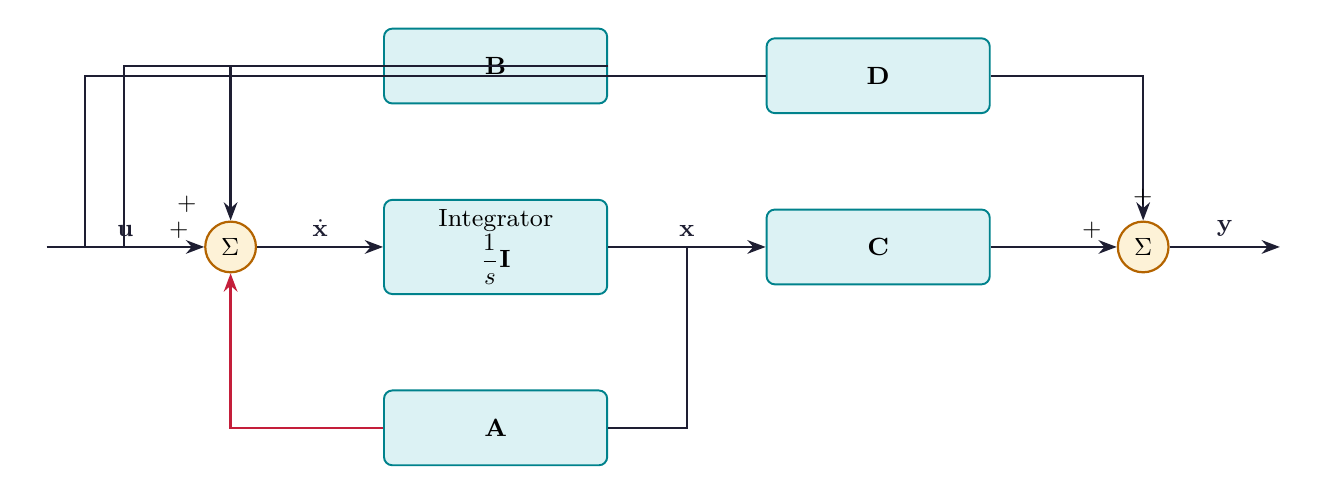
\begin{tikzpicture}[node distance=0.6cm and 1.4cm]
  % Main forward path nodes
  \node[sumjunc] (sum) {$\Sigma$};
  \node[block, right=1.6cm of sum] (int) {Integrator\\$\dfrac{1}{s}\mathbf{I}$};
  \node[block, right=2.0cm of int] (C) {$\mathbf{C}$};
  \node[sumjunc, right=1.6cm of C] (osum) {$\Sigma$};
  % Input / output terminals
  \node[left=2.0cm of sum] (u) {};
  \node[right=1.4cm of osum] (y) {};
  % A feedback block (below integrator)
  \node[block, below=1.2cm of int] (A) {$\mathbf{A}$};
  % B block (above integrator, between sum and int)
  \node[block, above=1.2cm of int] (B) {$\mathbf{B}$};
  % D block (above C, feedthrough)
  \node[block, above=1.2cm of C] (D) {$\mathbf{D}$};

  % ── Main signal path ──────────────────────────────────────────────────────
  \draw[arrow] (u)   -- node[above]{\small $\mathbf{u}$} (sum);
  \draw[arrow] (sum) -- node[above]{\small $\dot{\mathbf{x}}$} (int);
  \draw[arrow] (int) -- node[above]{\small $\mathbf{x}$} (C);
  \draw[arrow] (C)   -- (osum);
  \draw[arrow] (osum)-- node[above]{\small $\mathbf{y}$} (y);

  % ── B path: tap from input wire → B block → sum (top) ────────────────────
  \coordinate (utap) at ($(u)!0.45!(sum)$);
  \draw[line]  (utap) |- (B.west);
  \draw[arrow] (B.east) -| (sum.north);

  % ── D path: tap from input wire → D block → output sum (top) ─────────────
  \coordinate (utap2) at ($(u)!0.25!(sum)$);
  \draw[line]  (utap2) |- (D.west);
  \draw[arrow] (D.east) -| (osum.north);

  % ── A feedback: tap from x wire → A block → sum (south) ──────────────────
  \coordinate (xtap) at ($(int.east)!0.5!(C.west)$);
  \draw[line]     (xtap) |- (A.east);
  \draw[redarrow] (A.west) -| (sum.south);

  % ── Sign labels ───────────────────────────────────────────────────────────
  \node[above left=2pt and 2pt of sum]{\small $+$};
  \node[left=2pt of sum, yshift=6pt]{\small $+$};
  \node[above=2pt of osum]{\small $+$};
  \node[left=2pt of osum, yshift=6pt]{\small $+$};
\end{tikzpicture}
\end{tcolorbox}

\subsection{Choosing State Variables}

For a physical system, state variables are typically the \textbf{energy storage variables}:
\begin{itemize}[leftmargin=*, itemsep=2pt]
  \item \textbf{Electrical circuits:} Capacitor voltages $v_C$ and inductor currents $i_L$
  \item \textbf{Mechanical systems:} Displacement $x$ and velocity $\dot{x}$
  \item \textbf{Thermal systems:} Temperatures at each node
\end{itemize}

For an $n$-th order ODE, the standard choice is the \textbf{phase variable form}: $x_1 = y,\; x_2 = \dot{y},\; \ldots,\; x_n = y^{(n-1)}$.

\subsection{Phase Variable Form --- Example}

\begin{tcolorbox}[examplebox, title={Example: 3rd Order System}]
\textbf{Given ODE:} $\dddot{y} + a_2\ddot{y} + a_1\dot{y} + a_0 y = b_0 u$

\textbf{State variables:} $x_1 = y,\quad x_2 = \dot{y},\quad x_3 = \ddot{y}$

\textbf{State equations:}
\begin{align*}
\dot{x}_1 &= x_2 \\
\dot{x}_2 &= x_3 \\
\dot{x}_3 &= -a_0 x_1 - a_1 x_2 - a_2 x_3 + b_0 u
\end{align*}

\textbf{Matrix form:}
$$\begin{bmatrix}\dot{x}_1\\\dot{x}_2\\\dot{x}_3\end{bmatrix}
= \underbrace{\begin{bmatrix}0&1&0\\0&0&1\\-a_0&-a_1&-a_2\end{bmatrix}}_{\mathbf{A}}
\begin{bmatrix}x_1\\x_2\\x_3\end{bmatrix}
+ \underbrace{\begin{bmatrix}0\\0\\b_0\end{bmatrix}}_{\mathbf{B}} u, \qquad
y = \underbrace{\begin{bmatrix}1&0&0\end{bmatrix}}_{\mathbf{C}}\mathbf{x}$$

The $\mathbf{A}$ matrix in this form is called the \textbf{companion matrix} or \textbf{phase variable canonical form}.
\end{tcolorbox}

%═══════════════════════════════════════════════════════════════════════════════
\section{State Transition Matrix (STM)}
%═══════════════════════════════════════════════════════════════════════════════

\begin{tcolorbox}[defbox]
\textbf{State Transition Matrix (STM)} $\boldsymbol{\Phi}(t)$: Also called the \textbf{matrix exponential} $e^{\mathbf{A}t}$. It describes how the state vector transitions from its initial value $\mathbf{x}(0)$ to $\mathbf{x}(t)$ in the absence of any input (homogeneous case):
$$\mathbf{x}(t) = \boldsymbol{\Phi}(t)\,\mathbf{x}(0) = e^{\mathbf{A}t}\,\mathbf{x}(0)$$
\end{tcolorbox}

\subsection{Definition and Computation}

\begin{tcolorbox}[formulabox, title={Matrix Exponential --- Definition}]
$$\boldsymbol{\Phi}(t) = e^{\mathbf{A}t} = \mathbf{I} + \mathbf{A}t + \frac{\mathbf{A}^2 t^2}{2!} + \frac{\mathbf{A}^3 t^3}{3!} + \cdots = \sum_{k=0}^{\infty}\frac{(\mathbf{A}t)^k}{k!}$$
\end{tcolorbox}

\textbf{Methods to compute $e^{\mathbf{A}t}$:}

\begin{enumerate}[label=\textbf{\arabic*.}, leftmargin=*, itemsep=4pt]
  \item \textbf{Infinite series} (above) --- impractical for large $n$.
  \item \textbf{Laplace transform method:} $\boldsymbol{\Phi}(t) = \mathcal{L}^{-1}\{(s\mathbf{I}-\mathbf{A})^{-1}\}$
  \item \textbf{Cayley-Hamilton theorem:} Express $e^{\mathbf{A}t}$ as a polynomial in $\mathbf{A}$ of degree $\leq n-1$.
  \item \textbf{Diagonalisation:} If $\mathbf{A} = \mathbf{P}\mathbf{\Lambda}\mathbf{P}^{-1}$, then $e^{\mathbf{A}t} = \mathbf{P}\,e^{\mathbf{\Lambda}t}\,\mathbf{P}^{-1}$.
\end{enumerate}

\begin{tcolorbox}[formulabox, title={Laplace Method (Most Exam-Relevant)}]
$$\boldsymbol{\Phi}(t) = e^{\mathbf{A}t} = \mathcal{L}^{-1}\left\{(s\mathbf{I} - \mathbf{A})^{-1}\right\}$$
\textbf{Steps:}
\begin{enumerate}[label=\arabic*., leftmargin=*, itemsep=2pt, topsep=2pt]
  \item Form $(s\mathbf{I} - \mathbf{A})$ by subtracting $\mathbf{A}$ from $s$ times the identity matrix.
  \item Compute the inverse: $(s\mathbf{I} - \mathbf{A})^{-1} = \dfrac{\text{adj}(s\mathbf{I}-\mathbf{A})}{\det(s\mathbf{I}-\mathbf{A})}$
  \item Take the inverse Laplace transform of each element.
\end{enumerate}
\end{tcolorbox}

\subsection{Properties of the STM}

\begin{tabularx}{\linewidth}{|>{\centering\arraybackslash}p{0.6cm}|B{4.0cm}|X|}
\hline
\multicolumn{1}{|>{\centering\arraybackslash}p{0.6cm}|}{\textbf{\color{myteal}\#}} &
\multicolumn{1}{>{\centering\arraybackslash}p{4.0cm}|}{\textbf{\color{myteal}Property}} &
\multicolumn{1}{>{\centering\arraybackslash}X|}{\textbf{\color{myteal}Expression}} \\
\hline
1 & Initial value & $\boldsymbol{\Phi}(0) = \mathbf{I}$ (identity matrix) \\
\hline
2 & Inverse & $\boldsymbol{\Phi}^{-1}(t) = \boldsymbol{\Phi}(-t) = e^{-\mathbf{A}t}$ \\
\hline
3 & Composition & $\boldsymbol{\Phi}(t_1+t_2) = \boldsymbol{\Phi}(t_1)\,\boldsymbol{\Phi}(t_2)$ \\
\hline
4 & Derivative & $\dot{\boldsymbol{\Phi}}(t) = \mathbf{A}\,\boldsymbol{\Phi}(t) = \boldsymbol{\Phi}(t)\,\mathbf{A}$ \\
\hline
5 & Transition & $\boldsymbol{\Phi}(t_2 - t_1) = \boldsymbol{\Phi}(t_2)\,\boldsymbol{\Phi}^{-1}(t_1)$ \\
\hline
6 & Determinant & $\det[\boldsymbol{\Phi}(t)] = e^{\text{tr}(\mathbf{A})\cdot t} \neq 0$ (always non-singular) \\
\hline
\end{tabularx}

\begin{tcolorbox}[examplebox, title={Example: Compute STM for $\mathbf{A} = \begin{bmatrix}0&1\\-2&-3\end{bmatrix}$}]
$(s\mathbf{I}-\mathbf{A}) = \begin{bmatrix}s&-1\\2&s+3\end{bmatrix}$

$\det(s\mathbf{I}-\mathbf{A}) = s(s+3)+2 = s^2+3s+2 = (s+1)(s+2)$

$(s\mathbf{I}-\mathbf{A})^{-1} = \dfrac{1}{(s+1)(s+2)}\begin{bmatrix}s+3&1\\-2&s\end{bmatrix}$

Using partial fractions and inverse Laplace:
$$\boldsymbol{\Phi}(t) = \begin{bmatrix}2e^{-t}-e^{-2t} & e^{-t}-e^{-2t}\\-2e^{-t}+2e^{-2t} & -e^{-t}+2e^{-2t}\end{bmatrix}$$
\end{tcolorbox}

%═══════════════════════════════════════════════════════════════════════════════
\section{Solution of State Equations}
%═══════════════════════════════════════════════════════════════════════════════

\subsection{Homogeneous State Equation (Zero Input)}

When $\mathbf{u}(t) = \mathbf{0}$, the state equation reduces to:
$$\dot{\mathbf{x}}(t) = \mathbf{A}\,\mathbf{x}(t)$$

\begin{tcolorbox}[formulabox, title={Solution --- Homogeneous (Zero Input)}]
$$\boxed{\mathbf{x}(t) = e^{\mathbf{A}t}\,\mathbf{x}(0) = \boldsymbol{\Phi}(t)\,\mathbf{x}(0)}$$
This is the \textbf{free response} or \textbf{zero-input response}. It depends only on the initial state $\mathbf{x}(0)$ and the system matrix $\mathbf{A}$.\\[4pt]
The output is: $\mathbf{y}(t) = \mathbf{C}\,\boldsymbol{\Phi}(t)\,\mathbf{x}(0)$
\end{tcolorbox}

\textbf{Derivation:} Assume $\mathbf{x}(t) = e^{\mathbf{A}t}\mathbf{c}$. Then $\dot{\mathbf{x}} = \mathbf{A}e^{\mathbf{A}t}\mathbf{c} = \mathbf{A}\mathbf{x}$ ✓. At $t=0$: $\mathbf{x}(0) = \mathbf{c}$. Hence $\mathbf{x}(t) = e^{\mathbf{A}t}\mathbf{x}(0)$.

\subsection{Non-Homogeneous State Equation (With Input)}

When $\mathbf{u}(t) \neq \mathbf{0}$:
$$\dot{\mathbf{x}}(t) = \mathbf{A}\,\mathbf{x}(t) + \mathbf{B}\,\mathbf{u}(t)$$

\begin{tcolorbox}[formulabox, title={Solution --- Non-Homogeneous (With Input)}]
$$\boxed{\mathbf{x}(t) = \underbrace{e^{\mathbf{A}t}\,\mathbf{x}(0)}_{\text{zero-input}} + \underbrace{\int_0^t e^{\mathbf{A}(t-\tau)}\,\mathbf{B}\,\mathbf{u}(\tau)\,d\tau}_{\text{zero-state (convolution)}}}$$
$$= \boldsymbol{\Phi}(t)\,\mathbf{x}(0) + \int_0^t \boldsymbol{\Phi}(t-\tau)\,\mathbf{B}\,\mathbf{u}(\tau)\,d\tau$$
\textbf{Output:}
$$\mathbf{y}(t) = \mathbf{C}\,\boldsymbol{\Phi}(t)\,\mathbf{x}(0) + \int_0^t \mathbf{C}\,\boldsymbol{\Phi}(t-\tau)\,\mathbf{B}\,\mathbf{u}(\tau)\,d\tau + \mathbf{D}\,\mathbf{u}(t)$$
\end{tcolorbox}

\textbf{Derivation (variation of parameters):} Multiply both sides of $\dot{\mathbf{x}} - \mathbf{A}\mathbf{x} = \mathbf{B}\mathbf{u}$ by the integrating factor $e^{-\mathbf{A}t}$:
$$\frac{d}{dt}\left[e^{-\mathbf{A}t}\mathbf{x}(t)\right] = e^{-\mathbf{A}t}\mathbf{B}\mathbf{u}(t)$$
Integrating from $0$ to $t$ and multiplying by $e^{\mathbf{A}t}$ gives the result above.

\subsection{Laplace Domain Solution}

Taking the Laplace transform of $\dot{\mathbf{x}} = \mathbf{A}\mathbf{x} + \mathbf{B}\mathbf{u}$:

\begin{tcolorbox}[formulabox, title={Laplace Domain Solution}]
$$s\mathbf{X}(s) - \mathbf{x}(0) = \mathbf{A}\mathbf{X}(s) + \mathbf{B}\mathbf{U}(s)$$
$$(s\mathbf{I} - \mathbf{A})\mathbf{X}(s) = \mathbf{x}(0) + \mathbf{B}\mathbf{U}(s)$$
$$\mathbf{X}(s) = (s\mathbf{I}-\mathbf{A})^{-1}\mathbf{x}(0) + (s\mathbf{I}-\mathbf{A})^{-1}\mathbf{B}\mathbf{U}(s)$$
$$\mathbf{Y}(s) = \mathbf{C}(s\mathbf{I}-\mathbf{A})^{-1}\mathbf{x}(0) + \left[\mathbf{C}(s\mathbf{I}-\mathbf{A})^{-1}\mathbf{B} + \mathbf{D}\right]\mathbf{U}(s)$$
\end{tcolorbox}

%═══════════════════════════════════════════════════════════════════════════════
\section{Transfer Function from State Space}
%═══════════════════════════════════════════════════════════════════════════════

\begin{tcolorbox}[defbox]
The \textbf{transfer function matrix} $\mathbf{G}(s)$ relates the output $\mathbf{Y}(s)$ to the input $\mathbf{U}(s)$ with zero initial conditions $[\mathbf{x}(0) = \mathbf{0}]$:
$$\mathbf{G}(s) = \frac{\mathbf{Y}(s)}{\mathbf{U}(s)}\bigg|_{\mathbf{x}(0)=\mathbf{0}}$$
\end{tcolorbox}

\begin{tcolorbox}[formulabox, title={Transfer Function from State Space (Zero I.C.)}]
Setting $\mathbf{x}(0) = \mathbf{0}$ in the Laplace solution:
$$\mathbf{Y}(s) = \left[\mathbf{C}(s\mathbf{I}-\mathbf{A})^{-1}\mathbf{B} + \mathbf{D}\right]\mathbf{U}(s)$$
$$\boxed{\mathbf{G}(s) = \mathbf{C}(s\mathbf{I}-\mathbf{A})^{-1}\mathbf{B} + \mathbf{D}}$$
For SISO systems ($\mathbf{D}=0$ typically): $G(s) = \mathbf{C}(s\mathbf{I}-\mathbf{A})^{-1}\mathbf{B}$\\[4pt]
The \textbf{characteristic polynomial} is $\det(s\mathbf{I}-\mathbf{A})$, whose roots are the \textbf{eigenvalues} of $\mathbf{A}$ = poles of the system.
\end{tcolorbox}

\begin{tcolorbox}[examplebox, title={Example: TF from State Space}]
\textbf{Given:} $\mathbf{A}=\begin{bmatrix}0&1\\-2&-3\end{bmatrix}$, $\mathbf{B}=\begin{bmatrix}0\\1\end{bmatrix}$, $\mathbf{C}=\begin{bmatrix}1&0\end{bmatrix}$, $D=0$

$(s\mathbf{I}-\mathbf{A}) = \begin{bmatrix}s&-1\\2&s+3\end{bmatrix}$, \quad $\det = s^2+3s+2$

$(s\mathbf{I}-\mathbf{A})^{-1} = \dfrac{1}{s^2+3s+2}\begin{bmatrix}s+3&1\\-2&s\end{bmatrix}$

$G(s) = \mathbf{C}(s\mathbf{I}-\mathbf{A})^{-1}\mathbf{B} = \dfrac{1}{s^2+3s+2}\begin{bmatrix}1&0\end{bmatrix}\begin{bmatrix}s+3&1\\-2&s\end{bmatrix}\begin{bmatrix}0\\1\end{bmatrix} = \dfrac{1}{s^2+3s+2}$
\end{tcolorbox}

\begin{tcolorbox}[exambox, title={Exam Tips --- State Space \& STM}]
\begin{itemize}[leftmargin=*, itemsep=3pt, topsep=0pt]
  \item \textbf{STM} $= e^{\mathbf{A}t} = \mathcal{L}^{-1}\{(s\mathbf{I}-\mathbf{A})^{-1}\}$ --- Laplace method is fastest in exams.
  \item \textbf{Homogeneous solution:} $\mathbf{x}(t) = e^{\mathbf{A}t}\mathbf{x}(0)$ --- zero input, only initial state.
  \item \textbf{Non-homogeneous solution:} zero-input + zero-state (convolution integral).
  \item \textbf{TF from SS:} $G(s) = \mathbf{C}(s\mathbf{I}-\mathbf{A})^{-1}\mathbf{B} + \mathbf{D}$ --- set $\mathbf{x}(0)=\mathbf{0}$.
  \item \textbf{Poles} of the system = eigenvalues of $\mathbf{A}$ = roots of $\det(s\mathbf{I}-\mathbf{A})=0$.
  \item \textbf{$\boldsymbol{\Phi}(0) = \mathbf{I}$} always --- a quick check to verify your STM computation.
\end{itemize}
\end{tcolorbox}

%═══════════════════════════════════════════════════════════════════════════════
\section{Controllability}
%═══════════════════════════════════════════════════════════════════════════════

\begin{tcolorbox}[defbox]
\textbf{Controllability:} A system is said to be \textbf{completely state controllable} if it is possible to transfer the system from \textit{any} initial state $\mathbf{x}(t_0)$ to \textit{any} desired final state $\mathbf{x}(t_f)$ in a finite time $t_f - t_0$ using an unconstrained control input $\mathbf{u}(t)$.\\[4pt]
In simple terms: \textit{Can the input reach and control every state variable?}
\end{tcolorbox}

\subsection{Kalman's Controllability Test}

\begin{tcolorbox}[formulabox, title={Controllability Matrix}]
The system $(\mathbf{A}, \mathbf{B})$ is \textbf{completely controllable} if and only if the \textbf{controllability matrix} $\mathbf{Q}_c$ has full rank $n$:
$$\mathbf{Q}_c = \begin{bmatrix}\mathbf{B} & \mathbf{A}\mathbf{B} & \mathbf{A}^2\mathbf{B} & \cdots & \mathbf{A}^{n-1}\mathbf{B}\end{bmatrix}$$
$$\text{rank}(\mathbf{Q}_c) = n \quad \Leftrightarrow \quad \det(\mathbf{Q}_c) \neq 0 \quad \Leftrightarrow \quad \text{System is controllable}$$
$\mathbf{Q}_c$ is an $n \times nr$ matrix (for SISO: $n \times n$ square matrix).
\end{tcolorbox}

\begin{tcolorbox}[examplebox, title={Example: Check Controllability}]
\textbf{Given:} $\mathbf{A}=\begin{bmatrix}0&1\\-2&-3\end{bmatrix}$, $\mathbf{B}=\begin{bmatrix}0\\1\end{bmatrix}$, $n=2$

$\mathbf{A}\mathbf{B} = \begin{bmatrix}0&1\\-2&-3\end{bmatrix}\begin{bmatrix}0\\1\end{bmatrix} = \begin{bmatrix}1\\-3\end{bmatrix}$

$\mathbf{Q}_c = \begin{bmatrix}\mathbf{B} & \mathbf{A}\mathbf{B}\end{bmatrix} = \begin{bmatrix}0&1\\1&-3\end{bmatrix}$

$\det(\mathbf{Q}_c) = (0)(-3) - (1)(1) = -1 \neq 0$

\textbf{Result:} $\text{rank}(\mathbf{Q}_c) = 2 = n$ $\Rightarrow$ System is \textbf{completely controllable}.
\end{tcolorbox}

\subsection{Physical Interpretation}

\begin{itemize}[leftmargin=*, itemsep=3pt]
  \item If a system is \textbf{not controllable}, some state variables are \textit{decoupled} from the input --- no matter what $\mathbf{u}(t)$ is applied, those states cannot be driven to a desired value.
  \item \textbf{Pole placement} (assigning closed-loop poles arbitrarily) is possible \textit{only if} the system is completely controllable.
  \item An uncontrollable mode corresponds to a pole of the system that cannot be moved by state feedback.
\end{itemize}

%═══════════════════════════════════════════════════════════════════════════════
\section{Observability}
%═══════════════════════════════════════════════════════════════════════════════

\begin{tcolorbox}[defbox]
\textbf{Observability:} A system is said to be \textbf{completely observable} if every state variable $x_i(t_0)$ can be determined from the output $\mathbf{y}(t)$ over a finite time interval $[t_0, t_f]$, given the input $\mathbf{u}(t)$.\\[4pt]
In simple terms: \textit{Can we reconstruct every state variable by observing the output?}
\end{tcolorbox}

\subsection{Kalman's Observability Test}

\begin{tcolorbox}[formulabox, title={Observability Matrix}]
The system $(\mathbf{A}, \mathbf{C})$ is \textbf{completely observable} if and only if the \textbf{observability matrix} $\mathbf{Q}_o$ has full rank $n$:
$$\mathbf{Q}_o = \begin{bmatrix}\mathbf{C}\\\mathbf{C}\mathbf{A}\\\mathbf{C}\mathbf{A}^2\\\vdots\\\mathbf{C}\mathbf{A}^{n-1}\end{bmatrix}$$
$$\text{rank}(\mathbf{Q}_o) = n \quad \Leftrightarrow \quad \det(\mathbf{Q}_o) \neq 0 \quad \Leftrightarrow \quad \text{System is observable}$$
$\mathbf{Q}_o$ is an $mn \times n$ matrix (for SISO: $n \times n$ square matrix).
\end{tcolorbox}

\begin{tcolorbox}[examplebox, title={Example: Check Observability}]
\textbf{Given:} $\mathbf{A}=\begin{bmatrix}0&1\\-2&-3\end{bmatrix}$, $\mathbf{C}=\begin{bmatrix}1&0\end{bmatrix}$, $n=2$

$\mathbf{C}\mathbf{A} = \begin{bmatrix}1&0\end{bmatrix}\begin{bmatrix}0&1\\-2&-3\end{bmatrix} = \begin{bmatrix}0&1\end{bmatrix}$

$\mathbf{Q}_o = \begin{bmatrix}\mathbf{C}\\\mathbf{C}\mathbf{A}\end{bmatrix} = \begin{bmatrix}1&0\\0&1\end{bmatrix}$

$\det(\mathbf{Q}_o) = 1 \neq 0$

\textbf{Result:} $\text{rank}(\mathbf{Q}_o) = 2 = n$ $\Rightarrow$ System is \textbf{completely observable}.
\end{tcolorbox}

\subsection{Physical Interpretation}

\begin{itemize}[leftmargin=*, itemsep=3pt]
  \item If a system is \textbf{not observable}, some state variables are \textit{hidden} from the output --- they cannot be estimated from measurements.
  \item \textbf{State observer (Luenberger observer)} design is possible \textit{only if} the system is completely observable.
  \item An unobservable mode corresponds to a pole that does not appear in the transfer function (pole-zero cancellation).
\end{itemize}

\subsection{Controllability vs Observability --- Duality}

\begin{tcolorbox}[masonbox, title={Duality Principle (Kalman)}]
The system $(\mathbf{A}, \mathbf{B}, \mathbf{C})$ is \textbf{controllable} if and only if the \textbf{dual system} $(\mathbf{A}^T, \mathbf{C}^T, \mathbf{B}^T)$ is \textbf{observable}, and vice versa.\\[4pt]
This means: $\mathbf{Q}_c(\mathbf{A},\mathbf{B}) = \mathbf{Q}_o^T(\mathbf{A}^T,\mathbf{C}^T)$
\end{tcolorbox}

\begin{tabularx}{\linewidth}{|B{3.4cm}|>{\centering\arraybackslash}X|>{\centering\arraybackslash}X|}
\hline
\multicolumn{1}{|>{\centering\arraybackslash}p{3.4cm}|}{\textbf{Property}} &
\textbf{\color{myamber}Controllability} & \textbf{\color{mygreen}Observability} \\
\hline
Definition & Transfer any state to any other & Determine any state from output \\
\hline
Test matrix & $\mathbf{Q}_c = [\mathbf{B}\ \mathbf{A}\mathbf{B}\ \cdots\ \mathbf{A}^{n-1}\mathbf{B}]$ & $\mathbf{Q}_o = [\mathbf{C}^T\ (\mathbf{C}\mathbf{A})^T\ \cdots]^T$ \\
\hline
Condition & $\text{rank}(\mathbf{Q}_c) = n$ & $\text{rank}(\mathbf{Q}_o) = n$ \\
\hline
Matrices involved & $\mathbf{A}$ and $\mathbf{B}$ & $\mathbf{A}$ and $\mathbf{C}$ \\
\hline
Application & Pole placement, state feedback & State observer (Luenberger) \\
\hline
Dual of & Observability of $(\mathbf{A}^T, \mathbf{C}^T)$ & Controllability of $(\mathbf{A}^T, \mathbf{C}^T)$ \\
\hline
\end{tabularx}

\begin{tcolorbox}[exambox, title={Exam Tips --- Controllability \& Observability}]
\begin{itemize}[leftmargin=*, itemsep=3pt, topsep=0pt]
  \item \textbf{Controllability matrix:} $\mathbf{Q}_c = [\mathbf{B}\ \mathbf{A}\mathbf{B}\ \mathbf{A}^2\mathbf{B}\ \cdots\ \mathbf{A}^{n-1}\mathbf{B}]$ --- involves $\mathbf{A}$ and $\mathbf{B}$.
  \item \textbf{Observability matrix:} $\mathbf{Q}_o = [\mathbf{C}^T\ (\mathbf{C}\mathbf{A})^T\ \cdots\ (\mathbf{C}\mathbf{A}^{n-1})^T]^T$ --- involves $\mathbf{A}$ and $\mathbf{C}$.
  \item Both tests: compute the matrix, find its determinant. Non-zero $\Rightarrow$ full rank $\Rightarrow$ controllable/observable.
  \item \textbf{Pole-zero cancellation} in TF $\Rightarrow$ system is either uncontrollable or unobservable (or both).
  \item \textbf{Duality:} $(\mathbf{A},\mathbf{B})$ controllable $\Leftrightarrow$ $(\mathbf{A}^T,\mathbf{B}^T)$ observable.
  \item For a system in \textbf{phase variable form}: always controllable; observable depends on $\mathbf{C}$.
\end{itemize}
\end{tcolorbox}

%═══════════════════════════════════════════════════════════════════════════════
% QUICK REVISION --- MODULE 5
%═══════════════════════════════════════════════════════════════════════════════
\newpage
\begin{center}
  {\large\bfseries\color{myred} Quick Revision --- Module 5}\\[3pt]
  {\small\color{mydark} State Variable Analysis $|$ EC601}
\end{center}
\noindent{\color{myred}\rule{\linewidth}{1.2pt}}
\vspace{4pt}

\begin{tcolorbox}[formulabox, title={\textbf{Key Formulas at a Glance}}]
\begin{tabularx}{\linewidth}{B{5.2cm} X}
State equation              & $\dot{\mathbf{x}} = \mathbf{A}\mathbf{x} + \mathbf{B}\mathbf{u}$ \\[2pt]
Output equation             & $\mathbf{y} = \mathbf{C}\mathbf{x} + \mathbf{D}\mathbf{u}$ \\[2pt]
STM definition              & $\boldsymbol{\Phi}(t) = e^{\mathbf{A}t}$ \\[2pt]
STM via Laplace             & $\boldsymbol{\Phi}(t) = \mathcal{L}^{-1}\{(s\mathbf{I}-\mathbf{A})^{-1}\}$ \\[2pt]
STM series                  & $e^{\mathbf{A}t} = \mathbf{I} + \mathbf{A}t + \frac{\mathbf{A}^2t^2}{2!} + \cdots$ \\[2pt]
Homogeneous solution        & $\mathbf{x}(t) = e^{\mathbf{A}t}\mathbf{x}(0)$ \\[2pt]
Non-homogeneous solution    & $\mathbf{x}(t) = e^{\mathbf{A}t}\mathbf{x}(0) + \int_0^t e^{\mathbf{A}(t-\tau)}\mathbf{B}\mathbf{u}(\tau)\,d\tau$ \\[2pt]
Transfer function from SS   & $G(s) = \mathbf{C}(s\mathbf{I}-\mathbf{A})^{-1}\mathbf{B} + \mathbf{D}$ \\[2pt]
Characteristic polynomial   & $\det(s\mathbf{I}-\mathbf{A}) = 0$ \\[2pt]
Controllability matrix      & $\mathbf{Q}_c = [\mathbf{B}\ \mathbf{A}\mathbf{B}\ \cdots\ \mathbf{A}^{n-1}\mathbf{B}]$ \\[2pt]
Controllable condition      & $\text{rank}(\mathbf{Q}_c) = n$ \\[2pt]
Observability matrix        & $\mathbf{Q}_o = [\mathbf{C}^T\ (\mathbf{C}\mathbf{A})^T\ \cdots\ (\mathbf{C}\mathbf{A}^{n-1})^T]^T$ \\[2pt]
Observable condition        & $\text{rank}(\mathbf{Q}_o) = n$ \\[2pt]
STM property                & $\boldsymbol{\Phi}(0) = \mathbf{I}$; $\boldsymbol{\Phi}^{-1}(t) = \boldsymbol{\Phi}(-t)$
\end{tabularx}
\end{tcolorbox}

\vspace{5pt}

\begin{tcolorbox}[defbox, title={\textbf{One-Line Definitions}}]
\begin{itemize}[leftmargin=*, itemsep=3pt, topsep=0pt]
  \item \textbf{State:} Minimum set of variables that, with input, completely determines future system behaviour.
  \item \textbf{State Variable:} Each member of the minimum set; $n$ variables for an $n$-th order system.
  \item \textbf{State Vector $\mathbf{x}$:} Column vector of all $n$ state variables.
  \item \textbf{State Space:} $n$-dimensional space with state variables as axes.
  \item \textbf{$\mathbf{A}$ matrix:} System/plant matrix ($n\times n$); its eigenvalues are the system poles.
  \item \textbf{$\mathbf{B}$ matrix:} Input matrix ($n\times r$); couples input to state derivatives.
  \item \textbf{$\mathbf{C}$ matrix:} Output matrix ($m\times n$); selects which states appear in output.
  \item \textbf{$\mathbf{D}$ matrix:} Direct transmission matrix; usually zero for physical systems.
  \item \textbf{STM $\boldsymbol{\Phi}(t)$:} Matrix exponential $e^{\mathbf{A}t}$; maps initial state to state at time $t$.
  \item \textbf{Homogeneous solution:} Zero-input response; $\mathbf{x}(t) = e^{\mathbf{A}t}\mathbf{x}(0)$.
  \item \textbf{Non-homogeneous solution:} Zero-input + zero-state (convolution with input).
  \item \textbf{Controllability:} Ability to drive any state to any desired value using input.
  \item \textbf{Observability:} Ability to determine any state from output measurements.
  \item \textbf{Duality:} $(\mathbf{A},\mathbf{B})$ controllable $\Leftrightarrow$ $(\mathbf{A}^T,\mathbf{C}^T)$ observable.
\end{itemize}
\end{tcolorbox}

\vspace{5pt}

\begin{tcolorbox}[exambox, title={\textbf{Frequently Asked / Viva Questions}}]
\begin{enumerate}[topsep=0pt, label=\textbf{Q\arabic*.}, itemsep=5pt]
  \item \Q{What is a state variable?}
    The minimum set of variables that, together with the input, completely determines the future behaviour of the system. An $n$-th order system has exactly $n$ state variables.
  \item \Q{What is the State Transition Matrix?}
    $\boldsymbol{\Phi}(t) = e^{\mathbf{A}t}$. It maps the initial state to the state at time $t$ in the absence of input: $\mathbf{x}(t) = \boldsymbol{\Phi}(t)\mathbf{x}(0)$.
  \item \Q{How is the STM computed using Laplace transform?}
    $\boldsymbol{\Phi}(t) = \mathcal{L}^{-1}\{(s\mathbf{I}-\mathbf{A})^{-1}\}$. Form $(s\mathbf{I}-\mathbf{A})$, invert it, then take the inverse Laplace of each element.
  \item \Q{What is the solution of the homogeneous state equation?}
    $\mathbf{x}(t) = e^{\mathbf{A}t}\mathbf{x}(0)$. This is the zero-input (free) response depending only on the initial state.
  \item \Q{What is the solution of the non-homogeneous state equation?}
    $\mathbf{x}(t) = e^{\mathbf{A}t}\mathbf{x}(0) + \int_0^t e^{\mathbf{A}(t-\tau)}\mathbf{B}\mathbf{u}(\tau)\,d\tau$. Sum of zero-input and zero-state (convolution) responses.
  \item \Q{How is the transfer function obtained from state space?}
    Set $\mathbf{x}(0)=\mathbf{0}$ and take Laplace transform: $G(s) = \mathbf{C}(s\mathbf{I}-\mathbf{A})^{-1}\mathbf{B} + \mathbf{D}$.
  \item \Q{What are the poles of a state space system?}
    The eigenvalues of the $\mathbf{A}$ matrix, i.e., roots of $\det(s\mathbf{I}-\mathbf{A})=0$ (characteristic equation).
  \item \Q{Define controllability and state its test.}
    A system is controllable if any state can be driven to any desired state in finite time. Test: $\text{rank}(\mathbf{Q}_c) = n$ where $\mathbf{Q}_c = [\mathbf{B}\ \mathbf{A}\mathbf{B}\ \cdots\ \mathbf{A}^{n-1}\mathbf{B}]$.
  \item \Q{Define observability and state its test.}
    A system is observable if every state can be determined from the output in finite time. Test: $\text{rank}(\mathbf{Q}_o) = n$ where $\mathbf{Q}_o = [\mathbf{C}^T\ (\mathbf{C}\mathbf{A})^T\ \cdots]^T$.
  \item \Q{What is the duality principle?}
    $(\mathbf{A},\mathbf{B})$ is controllable if and only if $(\mathbf{A}^T,\mathbf{B}^T)$ is observable. Controllability and observability are dual concepts.

  \item \Q{What does pole-zero cancellation in TF indicate?}
    It indicates the system is either uncontrollable or unobservable (or both). The cancelled pole is a mode that is decoupled from either the input or the output.
  \item \Q{What are the properties of the STM?}
    \begin{itemize}[leftmargin=*, itemsep=1pt, topsep=2pt]
      \item $\boldsymbol{\Phi}(0) = \mathbf{I}$ (identity at $t=0$)
      \item $\boldsymbol{\Phi}^{-1}(t) = \boldsymbol{\Phi}(-t)$
      \item $\boldsymbol{\Phi}(t_1+t_2) = \boldsymbol{\Phi}(t_1)\,\boldsymbol{\Phi}(t_2)$
      \item $\dot{\boldsymbol{\Phi}}(t) = \mathbf{A}\,\boldsymbol{\Phi}(t)$
    \end{itemize}
\end{enumerate}
\end{tcolorbox}

\vspace{5pt}

\begin{tcolorbox}[tikzbox, title={\textbf{State Space Matrices --- Quick Reference}}]
\begin{tabularx}{\linewidth}{|>{\centering\arraybackslash}p{1.0cm}|>{\centering\arraybackslash}p{1.8cm}|>{\centering\arraybackslash}X|>{\raggedright\arraybackslash}X|}
\hline
\textbf{\color{myteal}Matrix} & \textbf{\color{myteal}Size} &
\multicolumn{1}{>{\centering\arraybackslash}X|}{\textbf{\color{myteal}Name}} &
\multicolumn{1}{>{\centering\arraybackslash}X|}{\textbf{\color{myteal}Role}} \\
\hline
$\mathbf{A}$ & $n \times n$ & System matrix & Governs state dynamics; eigenvalues = poles \\
\hline
$\mathbf{B}$ & $n \times r$ & Input matrix & Couples input to state derivatives \\
\hline
$\mathbf{C}$ & $m \times n$ & Output matrix & Selects states visible in output \\
\hline
$\mathbf{D}$ & $m \times r$ & Feedthrough matrix & Direct input-to-output path (usually $\mathbf{0}$) \\
\hline
$\mathbf{Q}_c$ & $n \times nr$ & Controllability matrix & Full rank $\Rightarrow$ controllable \\
\hline
$\mathbf{Q}_o$ & $mn \times n$ & Observability matrix & Full rank $\Rightarrow$ observable \\
\hline
\end{tabularx}
\end{tcolorbox}

\end{document}
